\documentclass{article}

\usepackage{ragged2e}
\usepackage{graphicx}
\usepackage{amsmath}
\usepackage{siunitx}

\begin{document}

\begin{flushright}
    \noindent
    Rodrigo Becerril Ferreyra\\
    CECS 211 Section 01\\
    Lab 4\\
    2019-10-10--2019-10-22
\end{flushright}

\indent
In this lab, we are tasked with finding the Thevenin and Norton
equivalent circuits for a certain given circuit, and verifying
if they act the same. Here is the circuit we will be
solving for:

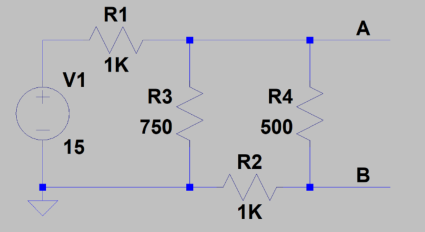
\includegraphics{Images/circuit0.png}

\section{Finding the Thevenin-Equivalent Circuit} The
Thevenin-equivalent circuit has two parts: the Thevenin
volatage and the Thevenin resistance. Each must be found
separately.

\subsection{Thevenin Voltage} The Thevenin voltage is found
by figuring out the voltage drop between terminals A and B.
To do this, we need to find the total current, and to do
this we need to find the equivalent resistance of the
circuit.

\begin{align*}
    R_{\text{net}}
    &= (R_4 + R_2) \parallel R_3 + R_1 \\
    &= (\SI{500}{\ohm} + \SI{1000}{\ohm}) \parallel \SI{750}{\ohm} + \SI{1000}{\ohm}\\
    &= \SI{1500}{\ohm} \parallel \SI{750}{\ohm} + \SI{1000}{\ohm}\\
    &= \SI{500}{\ohm} + \SI{1000}{\ohm} \\
    &= \SI{1.5}{\kilo\ohm}
\end{align*}

\pagebreak

Since Ohm's Law says that \(I = V/R\), the total current
going through this circuit is

\begin{align*}
    I_{\text{net}}
    &= V_1/R_{\text{net}}\\
    &= \SI{15}{\volt} / \SI{1.5}{\kilo\ohm}\\
    &= \SI{10}{\milli\ampere}
\end{align*}

Knowing the total current going through the circuit, we can
calculate the voltage drops across the resistors. The voltage
drop across \(R_1\) is \(\SI{10}{\milli\ampere} \cdot \SI{1}{\kilo\ohm}
= \SI{10}{\volt}\). That means that the voltage drop across
\(R_3\) is \SI{5}{\volt}. \(V_{R_2} + V_{R_4}\) must equal
\SI{5}{\volt} because the two combined are in parallel with
\(R_3\).

The current going across \(R_3\) is
\(\SI{5}{\volt}\cdot \SI{0.75}{\kilo\ohm} = \SI{6.667}{\milli\ampere}\).
By KCL, the current going through both \(R_4\) and \(R_2\) is
\( I_\text{net} - I_{R_3} = \SI{10}{\milli\ampere} - \SI{6.667}{\milli\ampere}
= \SI{3.333}{\milli\ampere}\); thus, the voltage going across
\(R_4\) and also the voltage from A to B is
\(\SI{0.5}{\kilo\ohm} \cdot \SI{3.333}{\milli\ampere} = \SI{1.667}{\volt}\)

With this, we can see our Thevenin-equivalent voltage is
\(V_{\text{Th}} = \SI{1.667}{\volt}\).

\subsection{Thevenin Resistance} The Thevenin resistance is the
resistance as seen from terminals A and B with all voltage
sources shorted out. In this example, voltage source \(V_1\)
is shorted out and replaced with a wire. This leaves \(R_1\) in
parallel with \(R_3\), and that is in series with \(R_2\), and
the whole thing is in parallel with \(R_4\):

\begin{align*}
    R_\text{Th}
    &= (R_1 \parallel R_3 + R_2) \parallel R_4\\
    &= (\SI{1000}{\ohm} \parallel \SI{750}{\ohm} + \SI{1000}{\ohm}) \parallel \SI{500}{\ohm}\\
    &= \SI{10000/7}{\ohm} \parallel \SI{500}{\ohm}\\
    &= \SI{10000/27}{\ohm} \approx \SI{370.37}{\ohm}
\end{align*}

Our Thevenin-equivalent resistance is \SI{370.37}{\ohm}.

\pagebreak

\subsection{Schematic} The schematic for this Thevenin-equivalent
circuit is as follows:

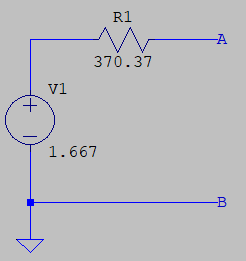
\includegraphics{Images/Thevenin.png}

\section{Adding a Load Resistor to the Original Circuit} To
verify that the original circuit and the Thevenin-equivalent
circuit are indeed equivalent, we will add a resistor of
value \SI{1000}{\ohm} (named \(R_L\)) connected to
terminals A and B. If the two circuits are indeed equivalent,
then both the voltage across \(R_L\) and the current going
through \(R_L\) should be equivalent across both circuits.

Adding \(R_L\) to the original circuit looks as follows:

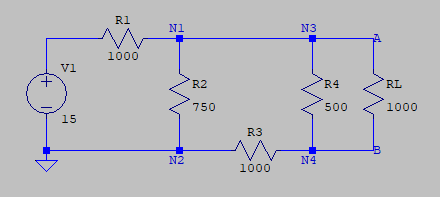
\includegraphics{Images/circuit0_RL.png}

Adding this new load resistor
transforms the original circuit into a completely new one.
In order to find the voltage across and current going through
this new circuit, we will need to find the new equivalent
resistance. Here, \(R_L\) and \(R_4\) are in parallel, and
combined are in series with \(R_3\). All of the previous
are in parallel with \(R_2\) which is in series with \(R_1\).
After we get the equivalent resistance of the circuit,
we can obtain the total current running through it.

\begin{align*}
    R_\text{net}
    &= (R_L \parallel R_4 + R_3) \parallel R_2 + R_1\\
    &= (\SI{1000}{\ohm} \parallel \SI{500}{\ohm} + \SI{1000}{\ohm}) \parallel \SI{750}{\ohm} + \SI{1000}{\ohm}\\
    &= \SI{4000/3}{\ohm} \parallel \SI{750}{\ohm} + \SI{1000}{\ohm}\\
    &= \SI{1480}{\ohm}
\end{align*}

\begin{align*}
    I_\text{net}
    &= V_1 / R_\text{net} = \SI{15}{\volt} / \SI{1480}{\ohm}\\
    &= \SI{3/296}{\ampere} \approx \SI{10.135}{\milli\ampere}
\end{align*}

The voltage across \(R_1\) is
\(R_1 \cdot I_\text{net} = \SI{1}{\kilo\ohm} \cdot \SI{10.135}{\milli\ampere} = \SI{10.135}{\volt}\).
This means that the voltage at Node 1 (\(N_1\)) is
\(\SI{15}{\volt} - \SI{10.135}{\volt} = \SI{4.865}{\volt}\)
(with respect to ground) and the voltage at
\(N_2 = \SI{0}{\volt}\); thus, the voltage across \(R_2\)
is \SI{4.865}{\volt}.
The current going through \(R_2\) is given
by \(V_{R_2}/R_2 = \SI{4.865}{\volt} / \SI{0.750}{\kilo\ohm}
\approx \SI{6.487}{\milli\ampere}\).

Because voltage is the same for every element in parallel, and
the combined resistance \((R_L \parallel R_4 + R_3)\) is all
in parallel with \(R_2\), that means that the voltage of the
combined resistance is \SI{4.865}{\volt}. The sum of the voltage of
\(R_4 = R_L\) and \(R_3\) must be equal to \SI{4.865}{\volt}
according to Kirchhoff's Voltage Law. The voltage of \(R_3\)
can be found %you can find voltage using current of the below commented-out text
using Kirchhoff's Current Law: 
the sum of currents entering any node must equal the sum
of currents exiting the node. In this case,
\(I_\text{net} = \SI{10.135}{\milli\ampere}\) is being summed
at \(N_2\) which is connected directly to the voltage source's
negative terminal. This means that the current leaving
\(N_2\) is equal to \(I_\text{net} = \SI{10.135}{\milli\ampere}\).
We know that the current going though \(R_2\) is
\SI{6.487}{\milli\ampere}.
This means that the current going through \(R_3\) must be

\begin{align*}
    I_{R_3}
    &= I_\text{net} - I_{R_2}\\
    &= \SI{10.135}{\milli\ampere} - \SI{6.487}{\milli\ampere}\\
    &= \SI{3.648}{\milli\ampere}
\end{align*}

With this value, we can find the voltage for \(R_3\):
\(V_{R_3} = \SI{1}{\kilo\ohm} \cdot \SI{3.648}{\milli\ampere}
= \SI{3.648}{\volt}\). This means that

\begin{align*}
    V_{R_4} = V_{R_L}
    &= V_{R_2} - V_{R_3}\\
    &= \SI{4.865}{\volt} - \SI{3.648}{\volt}\\
    &= \SI{1.217}{\volt}
\end{align*}

The voltage across \(R_L\) is \SI{1.217}{\volt}.

From this value of the voltage, the current can also be
calculated as follows:
\(I_{R_L} = V_{R_L} / R_L = \SI{1.217}{\volt} / \SI{1000}{\ohm}
= \SI{1.217}{\milli\ampere}\).

\section{Adding a Load Resistor to the Thevenin-Equivalent Circuit}
We will now verify that the values for the \(I_{R_L}\) and
\(V_{R_L}\) match for both circuits by solving the new Thevenin-
equivalent circuit when a load resistance of \SI{1000}{\ohm}
is added to it. The schematic for said circuit is as follows:

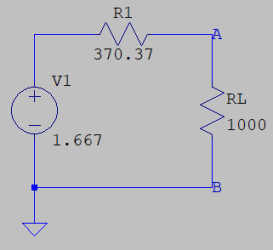
\includegraphics{Images/Thevenin_RL.png}

The total resistance of for this circuit is
\(R_\text{net} = R_1 + R_L = \SI{370.37}{\ohm} + \SI{1000}{\ohm}
= \SI{1370.37}{\ohm}\). The since this is a series circuit, the
total current going though the circuit is the same as the
current going through all components, including \(R_L\), and
that value is \(R_L = R_\text{net} = \SI{1.667}{\volt} / \SI{1370.37}{\ohm}
= \SI{1.216}{\milli\ampere}\). The voltage across the load
resistor is \(V_{R_L} = \SI{1.216}{\milli\ampere}\cdot\SI{1}{\kilo\ohm}
= \SI{1.216}{\volt}\). It clear to see that these values match
the values for the original circuit:

\begin{tabular}{c | c c}
            & Original & Thevenin \\ \hline
    Voltage & \SI{1.217}{\volt} & \SI{1.216}{\volt}\\
    Current & \SI{1.216}{\milli\ampere} & \SI{1.216}{\milli\ampere}
\end{tabular}

There was only an error of \(\pm \SI{0.001}{\volt}\) and
\(\pm \SI{0.001}{\milli\ampere}\) for the calculations of
voltage and current, respectively; this is only due to rounding.
These two circuits are indeed equivalent.

\pagebreak

\section{LTspice Simulation of Original Circuit} The original
circuit can be simulated in LTspice to acquire accurate
measured values for our load resistor with uncertainties
of \(\pm \SI{5}{\micro\volt}\) and \(\pm \SI{5}{\nano\ampere}\). The following are
the waveform and circuit for both voltage and current
of \(R_L\) of the original circuit:

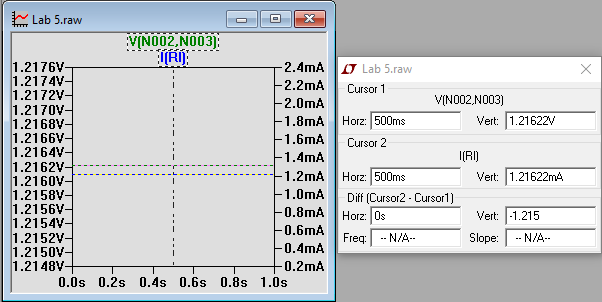
\includegraphics[width=\textwidth]{Images/circuit0_RL_Cursor.png}

In the waveform, the top line is the measured voltage,
and the bottom line is the measured current.

\section{Finding the Norton-Equivalent Circuit} Another
form of circuit simplification is Norton simplification.
Instead of acquiring an equivalent voltage, Norton simplification
finds an equivalent current. The way to find this equivalent
current is to short out terminals A and B, and find the current
between them. On a schematic, this would look as
follows\footnote{Note that when shorting out terminals A and B, the current
bypasses resistor \(R_4\), and it effectively disappears from
the circuit, as reflected in the above schematic.}:

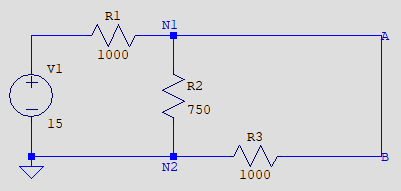
\includegraphics{Images/circuit0_short.png}

\subsection{Norton Current}
The current running through terminals A and B is the same
current running through resistor \(R_3\), so finding the
current through \(R_3\) will give us our Norton-equivalent current.

First, as always, it is necessary to find the equivalent resistance
of the new circuit. \(R_3\) is connected in parallel with
\(R_2\), and the two resistors are connected in series with
\(R_1\):

\begin{align*}
    R_\text{net}
    &= R_3 \parallel R_2 + R_1\\
    &= \SI{1000}{\ohm} \parallel \SI{750}{\ohm} + \SI{1000}{\ohm}\\
    &= \SI{0.428}{\kilo\ohm} + \SI{1000}{\ohm}\\
    &= \SI{1.428}{\kilo\ohm}
\end{align*}

The total current running though the circuit is
\(\SI{15}{\volt} / \SI{1.428}{\kilo\ohm} = \SI{10.50}{\milli\ampere}\).
The voltage across \(R_1\) is
\(\SI{10.50}{\milli\ampere}\cdot\SI{1}{\kilo\ohm} = \SI{10.50}{\volt}\).
This means that the voltage drop across \(R_2\) and \(R_3\) is
\SI{4.5}{\volt}. Therefore, the current going through
\(R_3\) and between terminals A and B is
\(\SI{4.5}{\volt} / \SI{1}{\kilo\ohm} = \SI{4.5}{\milli\ampere}\).
This is our Norton-equivalent current.

\subsection{Norton Resistance} Calculating the Norton-equivalent
resistance is the same process as calculating the Thevenin-
equivalent resistance, so we can reuse the value calculated
in Section 1.2, which is \SI{370.37}{\ohm}.

\subsection{Schematic} The schematic for the Norton-equivalent circuit
is as follows:

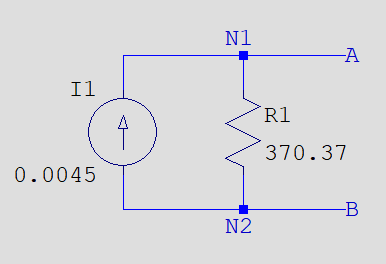
\includegraphics{Images/Norton.png}

\pagebreak

\section{Adding a Load Resistor to the Norton-Equivalent Circuit}

To verify that this circuit is also equivalent to both the
original circuit and the Thevenin-equivalent circuit, we will
be adding a load resistance of \(R_L = \SI{1000}{\ohm}\),
just like the Thevenin-equivalent circuit. The schematic
for this is as follows:

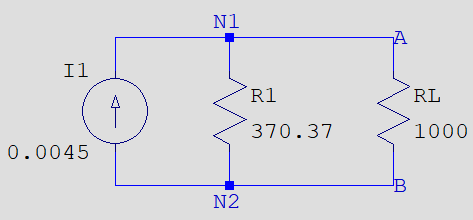
\includegraphics{Images/Norton_RL.png}

The equivalent resistance of the two resistors is simply
\(R_1 \parallel R_L\), or \SI{270.27}{\ohm}. The total
current going through the circuit is given by \(I_1\), which
is \SI{4.5}{\milli\ampere}, so the voltage across \(R_1\) and
\(R_L\) is \(\SI{4.5}{\milli\ampere}\cdot\SI{270.27}{\ohm}
= \SI{1.216}{\volt}\). The current going though \(R_l\) is
\(\SI{1.216}{\volt} / \SI{1}{\kilo\ohm} = \SI{1.216}{\milli\ampere}\).
As it is clear to see, these values corroborate with both
the original and Thevenin-equivalent circuits.

\section{Table of Values} This lab has clearly shown
that both Thevenin- and Norton-equivalent circuits are indeed
equivalent to the original circuit. I will end this report
with a table compiling the results of all the hand-calculated
values, as well as the values obtained by modeling every
circuit in LTspice.

\begin{tabular}[l]{l | l l l | l l l}
    
    & \multicolumn{3}{l|}{Hand Calculations} & \multicolumn{3}{l}{LTspice Model}\\ \hline
    & Original & Thevenin & Norton & Original & Thevenin & Norton\\ \hline
    Voltage & \SI{1.217}{\volt} & \SI{1.216}{\volt} & \SI{1.216}{\volt} & \SI{1.21622}{\volt} & \SI{1.21646}{\volt} & \SI{1.21622}{\volt}\\
    Current & \SI{1.217}{\milli\ampere} & \SI{1.216}{\milli\ampere} & \SI{1.216}{\milli\ampere} & \SI{1.21622}{\milli\ampere} & \SI{1.21646}{\milli\ampere} & \SI{1.21622}{\milli\ampere}

\end{tabular}

\end{document}
